The Plan and Execute Agent provides a deterministic, reproducible pipeline for answering questions via a strict plan of data-transform operations.

\begin{center}
  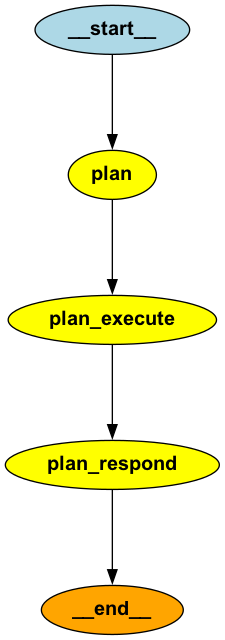
\includegraphics[width=0.13\textwidth]{graphics/graph-plan_and_execute.png}
  \captionof{figure}{Plan and Execute Agent Graph}
\end{center}

\begin{itemize}
  \item \textbf{Python mappings}: plan\_planner.py, plan\_executor.py, plan\_respond.py
  \item \textbf{Key schemas}: PlanToExecute, PlanExecuteFinalAnswer, Step types (from plan\_schemas.py), TraceEntry, DatasetEntry
  \item \textbf{Role}: Produce a deterministic plan (via plan\_planner), execute it (plan\_executor) against the dataset, and synthesize a final natural-language answer (plan\_respond).
  \item \textbf{How it operates}:
    \subitem Plan node (plan\_planner.py): receives the question and dataset paths; calls the LLM with PLANNER\_SYSTEM\_PROMPT to produce a strict JSON PlanToExecute, validating with PlanToExecute.model\_validate\_json. Returns plan\_execute\_result with plan and empty trace/execution\_result/final\_answer.
    \subitem Plan executor (plan\_executor.py): walks the plan's steps, applying each operation to the active DataFrame using plan\_operators.dispatch\_op, recording a trace of inputs/outputs and any errors. Supports snapshot/restore, joins, and concatenations via the DSL.
    \subitem Plan respond (plan\_respond.py): converts the final execution outcome into a PlanExecuteFinalAnswer using a dedicated LLM prompt that summarizes the execution and results.
  \item \textbf{Inputs}: state including question, csv\_paths, and dataset context; the planner's output is consumed by the executor.
  \item \textbf{Outputs}: PlanToExecute (from plan\_node), plan\_execute\_result (with final\_answer and trace), PlanExecuteFinalAnswer (for final natural-language answer).
  \item \textbf{Prompts design / structure}:
    \subitem The planner uses a DSL of operations: load\_dataset, select\_columns, rename\_columns, filter\_rows, derive\_columns, reduce\_columns, normalize\_columns, rank, group\_aggregate, sort\_rows, limit\_rows, distinct\_rows, pivot, snapshot, restore, join, concat, display.
    \subitem The plan\_node enforces the first step to be load\_dataset and uses a JSON structure for steps.
    \subitem plan\_executor uses plan\_operators to apply each Step to a DataFrame and records a trace for each step.
\end{itemize}
